%%%% fatec-article.tex, 2024/03/10

%% Classe de documento
\documentclass[
landscape,
  a4paper,%% Tamanho de papel: a4paper, letterpaper (^), etc.
  12pt,%% Tamanho de fonte: 10pt (^), 11pt, 12pt, etc.
  english,%% Idioma secundário (penúltimo) (>)
  brazilian,%% Idioma primário (último) (>)
]{article}

%% Pacotes utilizados
\usepackage[]{fatec-article}
\usepackage{setspace}

%% Processamento de entradas (itens) do índice remissivo (makeindex)
%\makeindex%

%% Arquivo(s) de referências
%\addbibresource{fatec-article.bib}

%% Início do documento
\begin{document}

% Seções e subseções
%\section{Título de Seção Primária}%

%\subsection{Título de Seção Secundária}%

%\subsubsection{Título de Seção Terciária}%

%\paragraph{Título de seção quaternária}%

%\subparagraph{Título de seção quinária}%

%\section*{Diário de Bordo}%

\break
 \begin{table}[H]
\centering
\begin{tabular}{|l|l|l|l|l|}
\hline

\multicolumn{1}{|c|}{Nome da Atividade} & \multicolumn{1}{c|}{Data de início} & \multicolumn{1}{c|}{Data de término} & \multicolumn{1}{c|}{\shortstack{Responsável \\ pela atividade}} & \multicolumn{1}{c|}{Descrição} \\
\hline
        Reunião de equipe: inicio das atividades  &  26 de Agosto  &    26 de Agosto          &  Elizama   & No dia 26 de Agosto, fizemos uma reunião de equipe e foi decidido que \tabularnewline & & &  & Eliana iria fazer as correções iniciais no artigo, traduzi-lo para o  \tabularnewline & & &  & inglês, e realizar as adaptações necessárias; Luiz e Carlos  \tabularnewline & & &  &ficariam responsáveis por desenvolver os protótipos e contribuir  \tabularnewline & & &  & na criação de artefatos de software; André iria programar as  \tabularnewline & & &  & interfaces faltantes, adicionar o projeto na nuvem AWS,  \tabularnewline & & &  &realizar testes com grande volume de dados e implementar  \tabularnewline & & &  &códigos para análises assintótica e de recorrência; Elizama  \tabularnewline & & &  & ficaria responsável pelo diário de bordo, correções no pitch,  \tabularnewline & & &  &gerenciamento da licença de software, e pela escrita e  \tabularnewline & & &  &documentação da AWS. Foi combinado que o prazo para a \tabularnewline & & &  &entrega   dessas atividades seria até o dia 20 de Outubro, faremos  \tabularnewline & & &  & outra reunião para acompanhar o andamento da segunda parte  \tabularnewline & & &  & do projeto. \\
        \\\hline

       
       
        

\end{tabular}
\end{table}

\newpage

                                    


% Inserir uma figura após a tabela

%\begin{photograph}[!h]


% Referenciar a figura no texto
\begin{figure}[h]
\caption{Evidência}
    \centering
    \begin{minipage}[t]{0.30\textwidth}
        \centering
        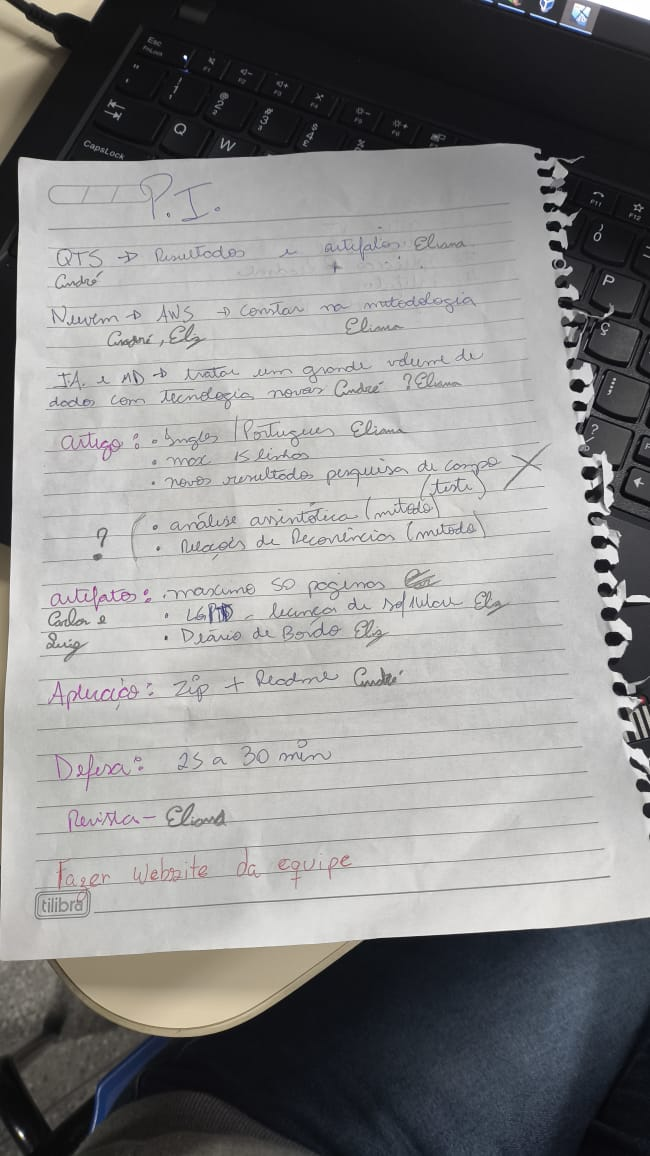
\includegraphics[width=\textwidth]{evidencias/img1.jpeg}
        \fonte{Autoria Própria (2024)}
        \label{fig:exemplo1}
    \end{minipage}
\end{figure}

\end{document}


